% Created by tikzDevice version 0.12.3.1 on 2022-05-11 22:51:23
% !TEX encoding = UTF-8 Unicode
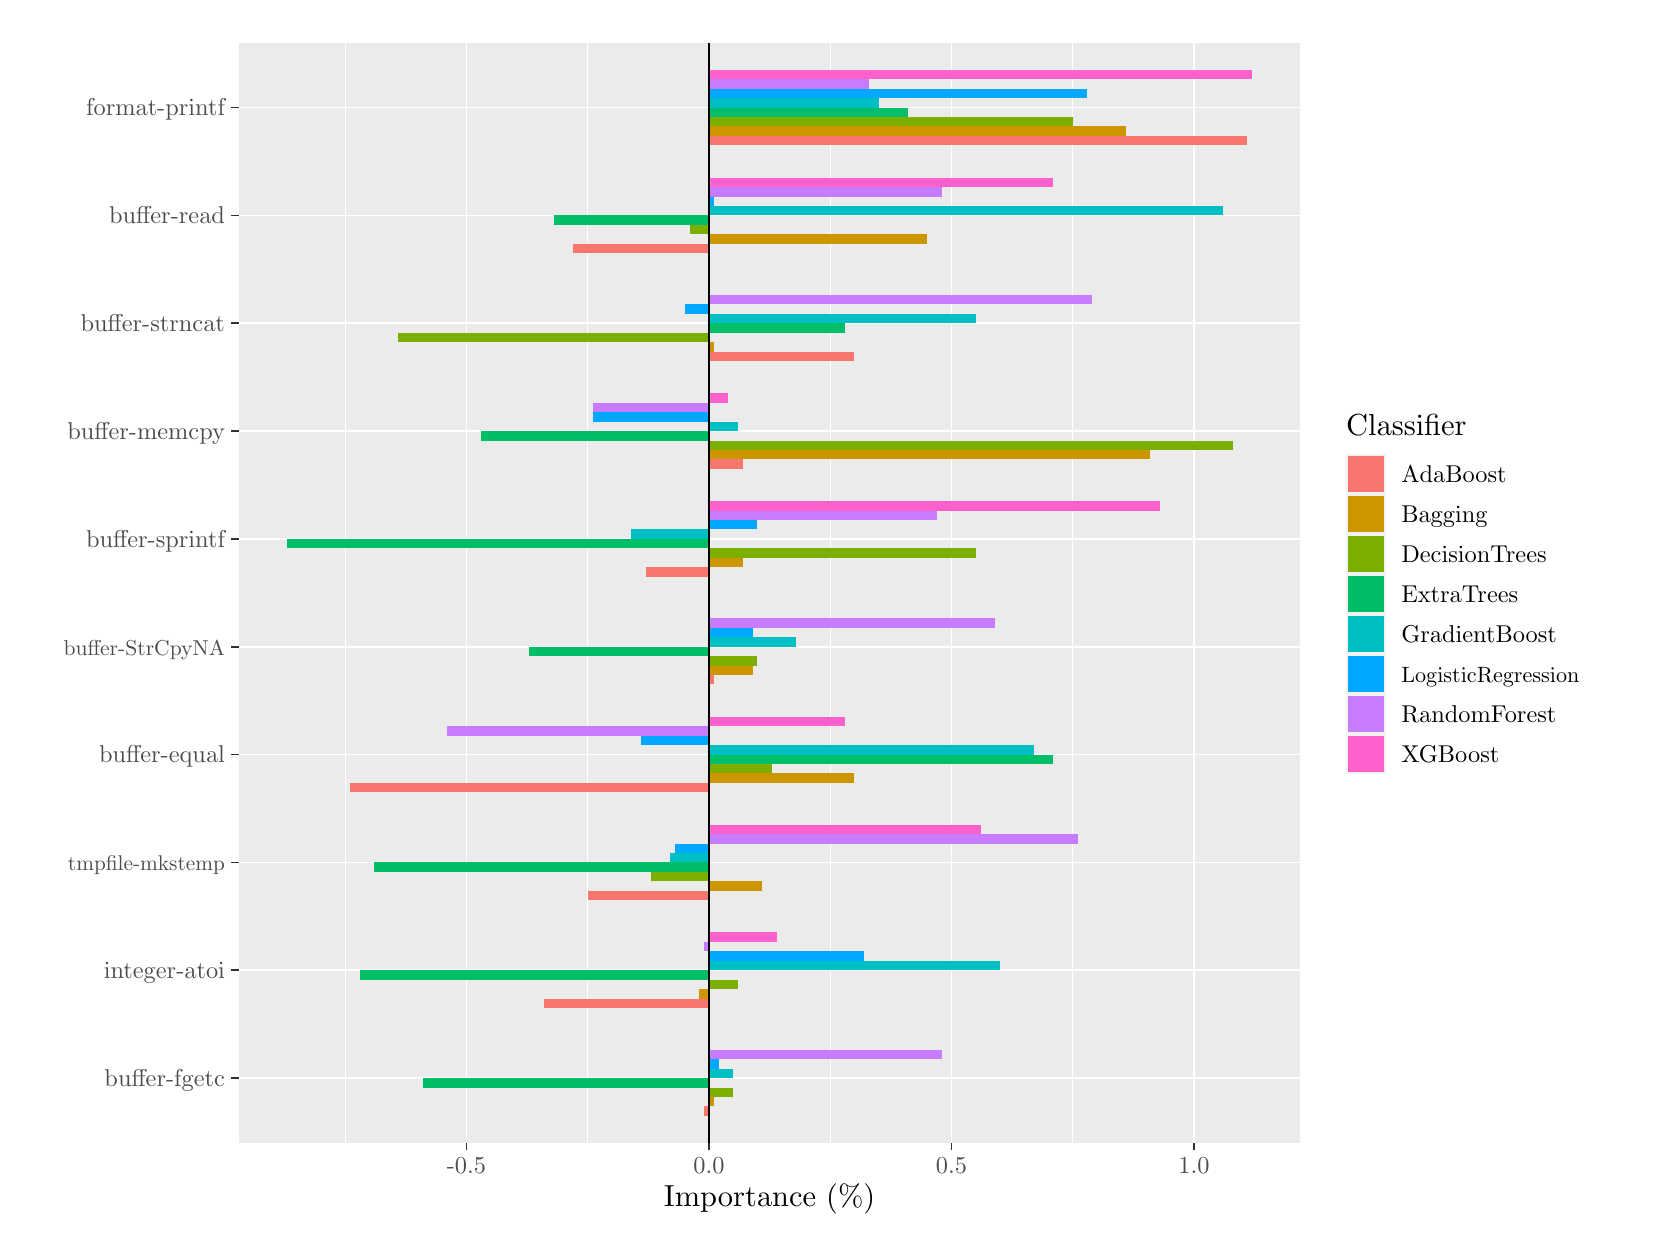
\begin{tikzpicture}[x=1pt,y=1pt]
\definecolor{fillColor}{RGB}{255,255,255}
\path[use as bounding box,fill=fillColor,fill opacity=0.00] (0,0) rectangle (578.16,433.62);
\begin{scope}
\path[clip] (  0.00,  0.00) rectangle (578.16,433.62);
\definecolor{drawColor}{RGB}{255,255,255}
\definecolor{fillColor}{RGB}{255,255,255}

\path[draw=drawColor,line width= 0.6pt,line join=round,line cap=round,fill=fillColor] (  0.00,  0.00) rectangle (578.16,433.62);
\end{scope}
\begin{scope}
\path[clip] ( 76.24, 30.69) rectangle (459.91,428.12);
\definecolor{fillColor}{gray}{0.92}

\path[fill=fillColor] ( 76.24, 30.69) rectangle (459.91,428.12);
\definecolor{drawColor}{RGB}{255,255,255}

\path[draw=drawColor,line width= 0.3pt,line join=round] (114.71, 30.69) --
	(114.71,428.12);

\path[draw=drawColor,line width= 0.3pt,line join=round] (202.35, 30.69) --
	(202.35,428.12);

\path[draw=drawColor,line width= 0.3pt,line join=round] (289.98, 30.69) --
	(289.98,428.12);

\path[draw=drawColor,line width= 0.3pt,line join=round] (377.62, 30.69) --
	(377.62,428.12);

\path[draw=drawColor,line width= 0.6pt,line join=round] ( 76.24, 54.06) --
	(459.91, 54.06);

\path[draw=drawColor,line width= 0.6pt,line join=round] ( 76.24, 93.03) --
	(459.91, 93.03);

\path[draw=drawColor,line width= 0.6pt,line join=round] ( 76.24,131.99) --
	(459.91,131.99);

\path[draw=drawColor,line width= 0.6pt,line join=round] ( 76.24,170.96) --
	(459.91,170.96);

\path[draw=drawColor,line width= 0.6pt,line join=round] ( 76.24,209.92) --
	(459.91,209.92);

\path[draw=drawColor,line width= 0.6pt,line join=round] ( 76.24,248.88) --
	(459.91,248.88);

\path[draw=drawColor,line width= 0.6pt,line join=round] ( 76.24,287.85) --
	(459.91,287.85);

\path[draw=drawColor,line width= 0.6pt,line join=round] ( 76.24,326.81) --
	(459.91,326.81);

\path[draw=drawColor,line width= 0.6pt,line join=round] ( 76.24,365.78) --
	(459.91,365.78);

\path[draw=drawColor,line width= 0.6pt,line join=round] ( 76.24,404.74) --
	(459.91,404.74);

\path[draw=drawColor,line width= 0.6pt,line join=round] (158.53, 30.69) --
	(158.53,428.12);

\path[draw=drawColor,line width= 0.6pt,line join=round] (246.16, 30.69) --
	(246.16,428.12);

\path[draw=drawColor,line width= 0.6pt,line join=round] (333.80, 30.69) --
	(333.80,428.12);

\path[draw=drawColor,line width= 0.6pt,line join=round] (421.44, 30.69) --
	(421.44,428.12);
\definecolor{fillColor}{RGB}{248,118,109}

\path[fill=fillColor] (246.16,391.10) rectangle (440.72,394.51);

\path[fill=fillColor] (197.09,352.14) rectangle (246.16,355.55);

\path[fill=fillColor] (246.16,313.18) rectangle (298.75,316.59);

\path[fill=fillColor] (246.16,274.21) rectangle (258.43,277.62);

\path[fill=fillColor] (223.38,235.25) rectangle (246.16,238.66);

\path[fill=fillColor] (246.16,196.28) rectangle (247.92,199.69);

\path[fill=fillColor] (116.46,157.32) rectangle (246.16,160.73);

\path[fill=fillColor] (202.35,118.36) rectangle (246.16,121.76);

\path[fill=fillColor] (186.57, 79.39) rectangle (246.16, 82.80);

\path[fill=fillColor] (244.41, 40.43) rectangle (246.16, 43.84);
\definecolor{fillColor}{RGB}{205,150,0}

\path[fill=fillColor] (246.16,394.51) rectangle (396.90,397.92);

\path[fill=fillColor] (246.16,355.55) rectangle (325.04,358.96);

\path[fill=fillColor] (246.16,316.59) rectangle (247.92,319.99);

\path[fill=fillColor] (246.16,277.62) rectangle (405.66,281.03);

\path[fill=fillColor] (246.16,238.66) rectangle (258.43,242.07);

\path[fill=fillColor] (246.16,199.69) rectangle (261.94,203.10);

\path[fill=fillColor] (246.16,160.73) rectangle (298.75,164.14);

\path[fill=fillColor] (246.16,121.76) rectangle (265.44,125.17);

\path[fill=fillColor] (242.66, 82.80) rectangle (246.16, 86.21);

\path[fill=fillColor] (246.16, 43.84) rectangle (247.92, 47.25);
\definecolor{fillColor}{RGB}{124,174,0}

\path[fill=fillColor] (246.16,397.92) rectangle (377.62,401.33);

\path[fill=fillColor] (239.15,358.96) rectangle (246.16,362.37);

\path[fill=fillColor] (133.99,319.99) rectangle (246.16,323.40);

\path[fill=fillColor] (246.16,281.03) rectangle (435.46,284.44);

\path[fill=fillColor] (246.16,242.07) rectangle (342.56,245.48);

\path[fill=fillColor] (246.16,203.10) rectangle (263.69,206.51);

\path[fill=fillColor] (246.16,164.14) rectangle (268.95,167.55);

\path[fill=fillColor] (225.13,125.17) rectangle (246.16,128.58);

\path[fill=fillColor] (246.16, 86.21) rectangle (256.68, 89.62);

\path[fill=fillColor] (246.16, 47.25) rectangle (254.93, 50.65);
\definecolor{fillColor}{RGB}{0,190,103}

\path[fill=fillColor] (246.16,401.33) rectangle (318.03,404.74);

\path[fill=fillColor] (190.08,362.37) rectangle (246.16,365.78);

\path[fill=fillColor] (246.16,323.40) rectangle (295.24,326.81);

\path[fill=fillColor] (163.79,284.44) rectangle (246.16,287.85);

\path[fill=fillColor] ( 93.68,245.48) rectangle (246.16,248.88);

\path[fill=fillColor] (181.31,206.51) rectangle (246.16,209.92);

\path[fill=fillColor] (246.16,167.55) rectangle (370.61,170.96);

\path[fill=fillColor] (125.23,128.58) rectangle (246.16,131.99);

\path[fill=fillColor] (119.97, 89.62) rectangle (246.16, 93.03);

\path[fill=fillColor] (142.75, 50.65) rectangle (246.16, 54.06);
\definecolor{fillColor}{RGB}{0,191,196}

\path[fill=fillColor] (246.16,404.74) rectangle (307.51,408.15);

\path[fill=fillColor] (246.16,365.78) rectangle (431.95,369.19);

\path[fill=fillColor] (246.16,326.81) rectangle (342.56,330.22);

\path[fill=fillColor] (246.16,287.85) rectangle (256.68,291.26);

\path[fill=fillColor] (218.12,248.88) rectangle (246.16,252.29);

\path[fill=fillColor] (246.16,209.92) rectangle (277.71,213.33);

\path[fill=fillColor] (246.16,170.96) rectangle (363.60,174.37);

\path[fill=fillColor] (232.14,131.99) rectangle (246.16,135.40);

\path[fill=fillColor] (246.16, 93.03) rectangle (351.33, 96.44);

\path[fill=fillColor] (246.16, 54.06) rectangle (254.93, 57.47);
\definecolor{fillColor}{RGB}{0,169,255}

\path[fill=fillColor] (246.16,408.15) rectangle (382.88,411.56);

\path[fill=fillColor] (246.16,369.19) rectangle (247.92,372.60);

\path[fill=fillColor] (237.40,330.22) rectangle (246.16,333.63);

\path[fill=fillColor] (204.10,291.26) rectangle (246.16,294.67);

\path[fill=fillColor] (246.16,252.29) rectangle (263.69,255.70);

\path[fill=fillColor] (246.16,213.33) rectangle (261.94,216.74);

\path[fill=fillColor] (221.63,174.37) rectangle (246.16,177.78);

\path[fill=fillColor] (233.90,135.40) rectangle (246.16,138.81);

\path[fill=fillColor] (246.16, 96.44) rectangle (302.25, 99.85);

\path[fill=fillColor] (246.16, 57.47) rectangle (249.67, 60.88);
\definecolor{fillColor}{RGB}{199,124,255}

\path[fill=fillColor] (246.16,411.56) rectangle (304.00,414.97);

\path[fill=fillColor] (246.16,372.60) rectangle (330.29,376.01);

\path[fill=fillColor] (246.16,333.63) rectangle (384.63,337.04);

\path[fill=fillColor] (204.10,294.67) rectangle (246.16,298.08);

\path[fill=fillColor] (246.16,255.70) rectangle (328.54,259.11);

\path[fill=fillColor] (246.16,216.74) rectangle (349.57,220.15);

\path[fill=fillColor] (151.52,177.78) rectangle (246.16,181.18);

\path[fill=fillColor] (246.16,138.81) rectangle (379.37,142.22);

\path[fill=fillColor] (244.41, 99.85) rectangle (246.16,103.26);

\path[fill=fillColor] (246.16, 60.88) rectangle (330.29, 64.29);
\definecolor{fillColor}{RGB}{255,97,204}

\path[fill=fillColor] (246.16,414.97) rectangle (442.47,418.38);

\path[fill=fillColor] (246.16,376.01) rectangle (370.61,379.41);

\path[fill=fillColor] (246.16,337.04) rectangle (246.16,340.45);

\path[fill=fillColor] (246.16,298.08) rectangle (253.17,301.49);

\path[fill=fillColor] (246.16,259.11) rectangle (409.17,262.52);

\path[fill=fillColor] (246.16,220.15) rectangle (246.16,223.56);

\path[fill=fillColor] (246.16,181.18) rectangle (295.24,184.59);

\path[fill=fillColor] (246.16,142.22) rectangle (344.32,145.63);

\path[fill=fillColor] (246.16,103.26) rectangle (270.70,106.67);

\path[fill=fillColor] (246.16, 64.29) rectangle (246.16, 67.70);
\definecolor{drawColor}{RGB}{0,0,0}

\path[draw=drawColor,line width= 0.6pt,line join=round] (246.16, 30.69) -- (246.16,428.12);
\end{scope}
\begin{scope}
\path[clip] (  0.00,  0.00) rectangle (578.16,433.62);
\definecolor{drawColor}{gray}{0.30}

\node[text=drawColor,anchor=base east,inner sep=0pt, outer sep=0pt, scale=  0.88] at ( 71.29, 51.03) {buffer-fgetc};

\node[text=drawColor,anchor=base east,inner sep=0pt, outer sep=0pt, scale=  0.88] at ( 71.29, 90.00) {integer-atoi};

\node[text=drawColor,anchor=base east,inner sep=0pt, outer sep=0pt, scale=  0.77] at ( 71.29,128.96) {tmpfile-mkstemp};

\node[text=drawColor,anchor=base east,inner sep=0pt, outer sep=0pt, scale=  0.88] at ( 71.29,167.93) {buffer-equal};

\node[text=drawColor,anchor=base east,inner sep=0pt, outer sep=0pt, scale=  0.78] at ( 71.29,206.89) {buffer-StrCpyNA};

\node[text=drawColor,anchor=base east,inner sep=0pt, outer sep=0pt, scale=  0.88] at ( 71.29,245.85) {buffer-sprintf};

\node[text=drawColor,anchor=base east,inner sep=0pt, outer sep=0pt, scale=  0.88] at ( 71.29,284.82) {buffer-memcpy};

\node[text=drawColor,anchor=base east,inner sep=0pt, outer sep=0pt, scale=  0.88] at ( 71.29,323.78) {buffer-strncat};

\node[text=drawColor,anchor=base east,inner sep=0pt, outer sep=0pt, scale=  0.88] at ( 71.29,362.75) {buffer-read};

\node[text=drawColor,anchor=base east,inner sep=0pt, outer sep=0pt, scale=  0.88] at ( 71.29,401.71) {format-printf};
\end{scope}
\begin{scope}
\path[clip] (  0.00,  0.00) rectangle (578.16,433.62);
\definecolor{drawColor}{gray}{0.20}

\path[draw=drawColor,line width= 0.6pt,line join=round] ( 73.49, 54.06) --
	( 76.24, 54.06);

\path[draw=drawColor,line width= 0.6pt,line join=round] ( 73.49, 93.03) --
	( 76.24, 93.03);

\path[draw=drawColor,line width= 0.6pt,line join=round] ( 73.49,131.99) --
	( 76.24,131.99);

\path[draw=drawColor,line width= 0.6pt,line join=round] ( 73.49,170.96) --
	( 76.24,170.96);

\path[draw=drawColor,line width= 0.6pt,line join=round] ( 73.49,209.92) --
	( 76.24,209.92);

\path[draw=drawColor,line width= 0.6pt,line join=round] ( 73.49,248.88) --
	( 76.24,248.88);

\path[draw=drawColor,line width= 0.6pt,line join=round] ( 73.49,287.85) --
	( 76.24,287.85);

\path[draw=drawColor,line width= 0.6pt,line join=round] ( 73.49,326.81) --
	( 76.24,326.81);

\path[draw=drawColor,line width= 0.6pt,line join=round] ( 73.49,365.78) --
	( 76.24,365.78);

\path[draw=drawColor,line width= 0.6pt,line join=round] ( 73.49,404.74) --
	( 76.24,404.74);
\end{scope}
\begin{scope}
\path[clip] (  0.00,  0.00) rectangle (578.16,433.62);
\definecolor{drawColor}{gray}{0.20}

\path[draw=drawColor,line width= 0.6pt,line join=round] (158.53, 27.94) --
	(158.53, 30.69);

\path[draw=drawColor,line width= 0.6pt,line join=round] (246.16, 27.94) --
	(246.16, 30.69);

\path[draw=drawColor,line width= 0.6pt,line join=round] (333.80, 27.94) --
	(333.80, 30.69);

\path[draw=drawColor,line width= 0.6pt,line join=round] (421.44, 27.94) --
	(421.44, 30.69);
\end{scope}
\begin{scope}
\path[clip] (  0.00,  0.00) rectangle (578.16,433.62);
\definecolor{drawColor}{gray}{0.30}

\node[text=drawColor,anchor=base,inner sep=0pt, outer sep=0pt, scale=  0.88] at (158.53, 19.68) {-0.5};

\node[text=drawColor,anchor=base,inner sep=0pt, outer sep=0pt, scale=  0.88] at (246.16, 19.68) {0.0};

\node[text=drawColor,anchor=base,inner sep=0pt, outer sep=0pt, scale=  0.88] at (333.80, 19.68) {0.5};

\node[text=drawColor,anchor=base,inner sep=0pt, outer sep=0pt, scale=  0.88] at (421.44, 19.68) {1.0};
\end{scope}
\begin{scope}
\path[clip] (  0.00,  0.00) rectangle (578.16,433.62);
\definecolor{drawColor}{RGB}{0,0,0}

\node[text=drawColor,anchor=base,inner sep=0pt, outer sep=0pt, scale=  1.10] at (268.07,  7.64) {Importance (\%)};
\end{scope}
\begin{scope}
\path[clip] (  0.00,  0.00) rectangle (578.16,433.62);
\definecolor{fillColor}{RGB}{255,255,255}

\path[fill=fillColor] (470.91,158.48) rectangle (572.66,300.33);
\end{scope}
\begin{scope}
\path[clip] (  0.00,  0.00) rectangle (578.16,433.62);
\definecolor{drawColor}{RGB}{0,0,0}

\node[text=drawColor,anchor=base west,inner sep=0pt, outer sep=0pt, scale=  1.10] at (476.41,286.18) {Classifier};
\end{scope}
\begin{scope}
\path[clip] (  0.00,  0.00) rectangle (578.16,433.62);
\definecolor{fillColor}{gray}{0.95}

\path[fill=fillColor] (476.41,265.16) rectangle (490.86,279.61);
\end{scope}
\begin{scope}
\path[clip] (  0.00,  0.00) rectangle (578.16,433.62);
\definecolor{fillColor}{RGB}{248,118,109}

\path[fill=fillColor] (477.12,265.87) rectangle (490.15,278.90);
\end{scope}
\begin{scope}
\path[clip] (  0.00,  0.00) rectangle (578.16,433.62);
\definecolor{fillColor}{gray}{0.95}

\path[fill=fillColor] (476.41,250.70) rectangle (490.86,265.16);
\end{scope}
\begin{scope}
\path[clip] (  0.00,  0.00) rectangle (578.16,433.62);
\definecolor{fillColor}{RGB}{205,150,0}

\path[fill=fillColor] (477.12,251.42) rectangle (490.15,264.45);
\end{scope}
\begin{scope}
\path[clip] (  0.00,  0.00) rectangle (578.16,433.62);
\definecolor{fillColor}{gray}{0.95}

\path[fill=fillColor] (476.41,236.25) rectangle (490.86,250.70);
\end{scope}
\begin{scope}
\path[clip] (  0.00,  0.00) rectangle (578.16,433.62);
\definecolor{fillColor}{RGB}{124,174,0}

\path[fill=fillColor] (477.12,236.96) rectangle (490.15,249.99);
\end{scope}
\begin{scope}
\path[clip] (  0.00,  0.00) rectangle (578.16,433.62);
\definecolor{fillColor}{gray}{0.95}

\path[fill=fillColor] (476.41,221.80) rectangle (490.86,236.25);
\end{scope}
\begin{scope}
\path[clip] (  0.00,  0.00) rectangle (578.16,433.62);
\definecolor{fillColor}{RGB}{0,190,103}

\path[fill=fillColor] (477.12,222.51) rectangle (490.15,235.54);
\end{scope}
\begin{scope}
\path[clip] (  0.00,  0.00) rectangle (578.16,433.62);
\definecolor{fillColor}{gray}{0.95}

\path[fill=fillColor] (476.41,207.34) rectangle (490.86,221.80);
\end{scope}
\begin{scope}
\path[clip] (  0.00,  0.00) rectangle (578.16,433.62);
\definecolor{fillColor}{RGB}{0,191,196}

\path[fill=fillColor] (477.12,208.05) rectangle (490.15,221.08);
\end{scope}
\begin{scope}
\path[clip] (  0.00,  0.00) rectangle (578.16,433.62);
\definecolor{fillColor}{gray}{0.95}

\path[fill=fillColor] (476.41,192.89) rectangle (490.86,207.34);
\end{scope}
\begin{scope}
\path[clip] (  0.00,  0.00) rectangle (578.16,433.62);
\definecolor{fillColor}{RGB}{0,169,255}

\path[fill=fillColor] (477.12,193.60) rectangle (490.15,206.63);
\end{scope}
\begin{scope}
\path[clip] (  0.00,  0.00) rectangle (578.16,433.62);
\definecolor{fillColor}{gray}{0.95}

\path[fill=fillColor] (476.41,178.43) rectangle (490.86,192.89);
\end{scope}
\begin{scope}
\path[clip] (  0.00,  0.00) rectangle (578.16,433.62);
\definecolor{fillColor}{RGB}{199,124,255}

\path[fill=fillColor] (477.12,179.15) rectangle (490.15,192.18);
\end{scope}
\begin{scope}
\path[clip] (  0.00,  0.00) rectangle (578.16,433.62);
\definecolor{fillColor}{gray}{0.95}

\path[fill=fillColor] (476.41,163.98) rectangle (490.86,178.43);
\end{scope}
\begin{scope}
\path[clip] (  0.00,  0.00) rectangle (578.16,433.62);
\definecolor{fillColor}{RGB}{255,97,204}

\path[fill=fillColor] (477.12,164.69) rectangle (490.15,177.72);
\end{scope}
\begin{scope}
\path[clip] (  0.00,  0.00) rectangle (578.16,433.62);
\definecolor{drawColor}{RGB}{0,0,0}

\node[text=drawColor,anchor=base west,inner sep=0pt, outer sep=0pt, scale=  0.88] at (496.36,269.35) {AdaBoost};
\end{scope}
\begin{scope}
\path[clip] (  0.00,  0.00) rectangle (578.16,433.62);
\definecolor{drawColor}{RGB}{0,0,0}

\node[text=drawColor,anchor=base west,inner sep=0pt, outer sep=0pt, scale=  0.88] at (496.36,254.90) {Bagging};
\end{scope}
\begin{scope}
\path[clip] (  0.00,  0.00) rectangle (578.16,433.62);
\definecolor{drawColor}{RGB}{0,0,0}

\node[text=drawColor,anchor=base west,inner sep=0pt, outer sep=0pt, scale=  0.88] at (496.36,240.45) {DecisionTrees};
\end{scope}
\begin{scope}
\path[clip] (  0.00,  0.00) rectangle (578.16,433.62);
\definecolor{drawColor}{RGB}{0,0,0}

\node[text=drawColor,anchor=base west,inner sep=0pt, outer sep=0pt, scale=  0.88] at (496.36,225.99) {ExtraTrees};
\end{scope}
\begin{scope}
\path[clip] (  0.00,  0.00) rectangle (578.16,433.62);
\definecolor{drawColor}{RGB}{0,0,0}

\node[text=drawColor,anchor=base west,inner sep=0pt, outer sep=0pt, scale=  0.88] at (496.36,211.54) {GradientBoost};
\end{scope}
\begin{scope}
\path[clip] (  0.00,  0.00) rectangle (578.16,433.62);
\definecolor{drawColor}{RGB}{0,0,0}

\node[text=drawColor,anchor=base west,inner sep=0pt, outer sep=0pt, scale=  0.80] at (496.36,197.08) {LogisticRegression};
\end{scope}
\begin{scope}
\path[clip] (  0.00,  0.00) rectangle (578.16,433.62);
\definecolor{drawColor}{RGB}{0,0,0}

\node[text=drawColor,anchor=base west,inner sep=0pt, outer sep=0pt, scale=  0.88] at (496.36,182.63) {RandomForest};
\end{scope}
\begin{scope}
\path[clip] (  0.00,  0.00) rectangle (578.16,433.62);
\definecolor{drawColor}{RGB}{0,0,0}

\node[text=drawColor,anchor=base west,inner sep=0pt, outer sep=0pt, scale=  0.88] at (496.36,168.18) {XGBoost};
\end{scope}
\end{tikzpicture}
